

\section{Introduction}

A memory allocator is a key component that could significantly impact the performance and memory consumption of the corresponding applications. We performed an experiment on applications of PARSEC~\cite{parsec}, and stress tests of Hoard~\cite{Hoard}, with multiple well-known memory allocators. These allocators include two versions of Linux allocators (glibc-2.28 and glibc-2.21), TcMalloc~\cite{tcmalloc}, \texttt{jemalloc}~\cite{jemalloc}, and Hoard~\cite{Hoard}, among them both TcMalloc and \texttt{jemalloc} are industrial level allocators. Figure~\ref{fig:motivation} shows performance results of partial programs, where all data in the figure is normalized to that of the Linux default allocator (glibc-2.28). We have the following observations: (1)~the performance difference with different allocators can be as large as $38\times$, i.e. \texttt{cache-thrash} with TcMalloc; (2)~No allocator performs consistently the best across all tested applications, indicating the importance of identifying the internal reason.
%, indicating that sometimes spending additional effort toward optimizing the application code may have a smaller  impact than simply switching to a better-suited allocator. (2)~No allocator performs consistently the best across all tested applications, indicating the importance of identifying the internal reason. 

\begin{figure}[!ht]
\centering
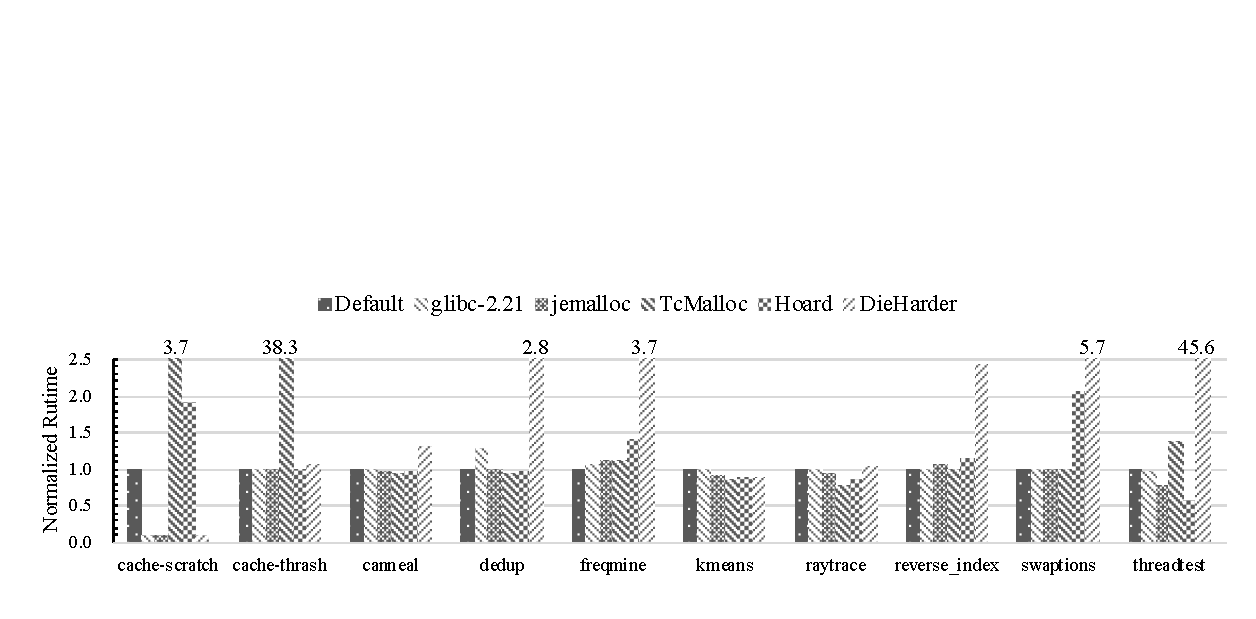
\includegraphics[width=0.98\columnwidth]{figures/perfdiff}
\caption{Performance Impact of Allocators\label{fig:motivation}}
\end{figure}

\begin{figure}[!ht]
\centering
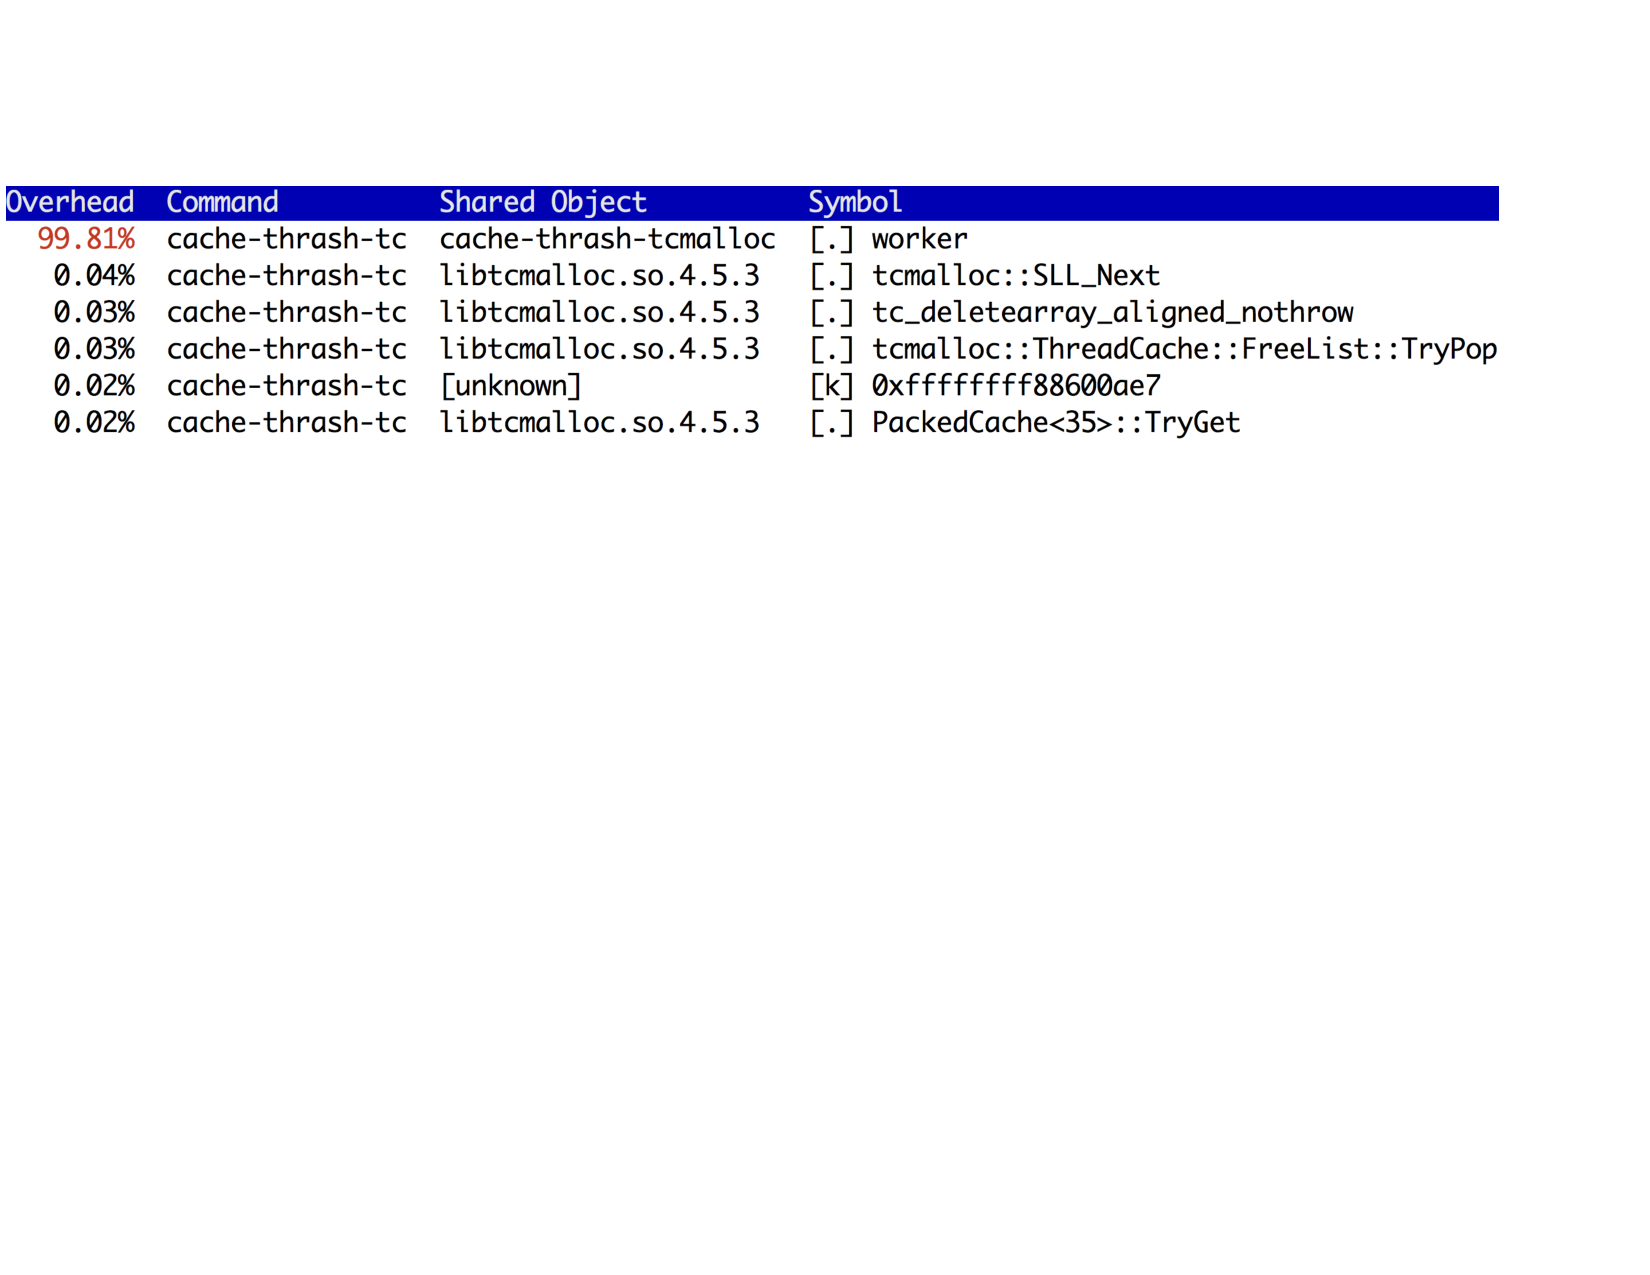
\includegraphics[width=0.9\columnwidth]{figures/perf-cache-thrash-tcmalloc}
\caption{Profiling results of \texttt{perf}. \label{fig:mot1}}
\end{figure}

However, none of existing profilers can identify the inherent reason of the performance slowdown caused by an allocator. General profilers, such as \texttt{gprof}~\cite{DBLP:conf/sigplan/GrahamKM82} and \texttt{perf}~\cite{perf}, only report the time accumulation of different functions, and \texttt{Coz}~\cite{Coz} presents a quantitative performance impact of improving a particular region of code. We used \texttt{perf}, \texttt{gprof}, and \texttt{Coz} to analyze the performance issue of TcMalloc on \texttt{cache-thrash}, since it runs around $38\times$ slower than the default Linux allocator. As shown in Figure~\ref{fig:mot1}, \texttt{perf} reports the \texttt{worker} function as the primary function to focus on, which unfortunately has nothing to do with the slowdown reason. \texttt{gprof} reports a similar result as \texttt{perf}. \texttt{Coz} reports reports the program lines of exercising these objects with passive false sharing issues, i.e. lines 85-87 of \texttt{cache-thrash.cpp}, and predicts that the performance can be improved up to \textbf{10\%} if these lines can be improved by 100\%. However, \texttt{Coz} does not pinpoint that the performance slowdown is actually caused by the allocator, as discussed in Section~\ref{sec:effectiveness}, and its prediction on the performance impact is obviously much smaller than the real one.

%However, they cannot identify the performance issues of a memory allocator, due to the following reasons. \texttt{First}, they do not collect allocator-specific data, and provide no metrics for evaluating an allocator. For instance, \texttt{perf} may report the number of cache misses, but it is impossible to know how many of these events are actually caused by the allocator. Without that information, it is unable to determine whether a performance issue is originating from the allocator. \texttt{Second}, none of these tools collect kernel contention information, an important issue related to the allocator. For instance, the glibc-2.21 allocator slows down the performance of \texttt{dedup} by more than 20\%, which is caused by frequent \texttt{madivse} system calls that directly lead to the heavy kernel contention. However, such an important issue cannot be identified by general profilers~\cite{DBLP:conf/sigplan/GrahamKM82, Coz, perf}%, \todo{as discussed in Section~\ref{}}.
%Third, none of these profilers report the application friendliness of an allocator, which is critical to understanding the performance slowdown caused by a particular allocator.   

Existing allocator profilers, such as \texttt{mprof}~\cite{Zorn:1988:MAP:894814}, Mtrace~\cite{mtrace}, Mtrace++~\cite{Lee:2000:DMM:786772.787150}, \texttt{TcMalloc} profiler~\cite{tcmalloc-profiler}, or CLR profiler~\cite{lupasc2014dynamic}, mainly focus on how an application uses the memory. For instance, \texttt{mprof} attributes memory allocations to different allocation sites, and reports memory leaks and a direct allocation table that shows the memory usage of functions~\cite{Zorn:1988:MAP:894814}. The \texttt{TcMalloc} profiler reports heap usage of different allocation sites, and locates memory leaks~\cite{tcmalloc-profiler}. That is, these allocation profilers cannot tell the design issues inside a particular allocator. 

Due to the obvious important impact of a memory allocator, it is emergent to design a profiler that could pinpoint design/implementation issues of an allocator. This profiler should be able to profile different allocators so that there is no need to reinvent the wheel for allocator designers, when they design a new allocator or improve an existing allocator. More importantly, the profiler should also benefit normal users, not just limit to allocator designers. This paper presents such a profiler--\MP{}--that focuses on different aspects of an allocator that will benefit both allocator designers and normal users. 

\MP{} will benefit normal users in the following ways. First, \MP{} can predict potential performance improvement when switching to an exemplar allocator (such as TcMalloc), which clearly indicates whether it is necessary to improve the allocator or switch to a new allocator. Second, \MP{} will report detailed memory wastes caused by an allocator, which is overlooked by existing profilers. Third, \MP{} will also report multiple application-friendliness metrics, which tells whether an allocator is tapped with allocation/deallocation pattern or access pattern of a particular application. As described above, a well-performed allocator like TcMalloc may be not suitable for a particular application (e.g., \texttt{cache-thrash}). Overall, \MP{} will provide a range of metrics on evaluating an allocator for normal users, not just limiting to the runtime. 
% which helps determine whether the current allocator is suitable for this application or not.

%\todo{Differentiation is important to know the details. }
\textit{The novelty (and challenge) of \MP{} lies in its decision of what to profile and how to profile precisely and efficiently}, as described in the following. First, \MP{} profiles the performance impact of memory management operations, which will directly affect the performance of running an application. It is straightforward to utilize the time (cycles) of each allocation and deallocation as the metrics, but there exist multiple issues. The first issue is that the summarized data is misleading (\textit{preciseness issue}), since there exist different types of allocations. For instance, an allocator typically handles small and big objects differently. The second issue is that the runtime itself cannot tell the underlying reason for the performance issue. Instead, \MP{} differentiates the data based on allocation types, such as small/large allocation, new/re-used allocation, which helps identify the real issue inside the allocator. In addition, \MP{} proposes to utilize hardware Performance Monitor Units (PMUs) to collect hardware related events (instructions, cache misses, or page faults), and intercept synchronizations and memory-related system calls to obtain user-space and kernel contention, helping understand the particular design issue inside. For instance, glibc-2.21 invokes a large number of \texttt{madvise} system calls for the \texttt{dedup} application~\cite{madvise}, where the system call overhead and unnecessary page faults are the major reason of 28\% slowdown. 
%\MP{} is able to report such issues by intercepting memory-related system calls. 

Second, \MP{} reports different types of memory wastes introduced by an allocator. It is straightforward to measure internal fragmentation of an allocator, which could be collected using the difference between a requested size with its corresponding class size. However, it is challenging to measure other wastes, such as memory blowup and external fragmentation. Memory blowup occurs when memory deallocations from one thread cannot be utilized to satisfy subsequent memory requests from other threads~\cite{Hoard}, due to the utilization of per-thread heaps. However, this definition cannot be utilized directly to collect the total memory blowup, as it does not specify how to update upon consequent deallocations and re-allocations. \MP{} computes memory blowup with a key observation: \textit{the total size of freed objects represent the upper bound of memory blowup for a size class}. Then the memory blowup can be computed by subtracting the total size with the size of recently-freed objects. After computing the memory blowup, \MP{} is able to compute the external fragmentation afterwards. 

Third, \MP{} will identify application-friendliness of an allocator, indicating whether an allocator is tapping well with memory usage pattern and access pattern of a particular application. Such application-friendliness include cache utilization rate, page utilization rate, passive/active false sharing, and cache invalidation rate (outside allocations/deallocations). \MP{} proposes to utilize hardware-based sampling in order to reduce the performance overhead. For instance, to collect cache utilization rate, \MP{} tracks used bytes of every cache line, and then updates the overall cache utilization rate upon every sampled access. Overall, these parameters will help users to understand the performance degradation on a specific application. For the previous example, \MP{} reports that the passive false sharing is the direct reason for TcMalloc's low performance on \texttt{cache-trash} application.

Overall, \MP{} profiles multiple important aspects of memory allocators, such as performance, memory, scalability, and application-friendliness. Based on our extensive evaluation, \MP{} successfully identifies multiple known and \textbf{un-known} design issues inside popular allocators, as further described in Section~\ref{sec:effectiveness}. Due to its careful design, \todo{\MP{}'s performance overhead is around $50\%$ and its memory overhead is around $56\%$}. This efficient design reduces \MP{}'s interference to the original execution. \MP{} does not need the change of the allocator, the application, and the underlying OS, which will be convenient for the employment. 

%\todo{one way to highlight the contribution is to emphasize on the **complex** considerations of designing good allocators and the challenges to identify design problems. We want to let the reviewer know that it's difficult to do. }

\subsection*{Contribution}

Overall, this paper makes the following contributions. 

\begin{itemize}
\item \MP{} is the first systematic approach to evaluate and profile different memory allocators, without changing the internal implementation of allocators. More specifically, \MP{} proposes the combination of function interception (based on common APIs) and PMU-based sampling to perform the profiling.

%It proposes the first general profiler--\MP{}--to profile different memory allocators, without the need of the change of the allocator and the underlying OS, if an allocator utilizes the standard synchronization and system calls.  

\item \MP{} presents a comprehensive study on relevant factors that an allocator may impact the performance of applications.
%important reasons that may impact  of an allocator that will significantly impact the performance and memory overhead of an allocator, with the assistance of PMUs, time-stamp counters, and simple counters together. 

\item \MP{} proposes the first mechanisms to quantitatively measure memory blowup (and external fragmentation), cache/page utilization rate, and passive/active false sharing impact. 
%, multiple practical methods to profile some metrics precisely and efficiently for the first time, such as memory blowup, . 
%profile cache/page utilization rate, memory blowup, active/passive false sharing, and kernel contention for the first time.
%, and attributes the data to each allocation and deallocation, helps discover designing issues that cannot be discovered with general profilers.  
%\item \MP{} proposes a practical method to predict the performance impact of the current allocator, which allows normal users to 
\item This paper performs extensive experimentation to confirm its effectiveness and overhead.    

\end{itemize} 

\begin{comment}

%\todo{What is new in this tool? Whether it could provide some information that is not available in an existing allocator.}

\begin{itemize}
\item It will quantify application-friendliness, which is not available in existing work, and which helps users to decide which allocator should be used for a specific application. 
\item It will provide the memory usage (overhead) information, such as internal fragmentation, and objects that are not freed but yet which remain unused. 
\item It will provide some information that only exists across multiple profilers, for instance, the average number of instructions of each allocation and deallocation, the average time spent within each allocation and deallocation (PMU sampling will be placed outside of the time span, thus not avoiding an erroneous measurement of how long this allocation and deallocation request has been sampled), whether there are some contentions during allocation (user space and kernel space), how many lock acquisitions.  
\end{itemize}
 	
\end{comment}

\subsection*{Outline}

The remained of this paper is organized as follows. Section~\ref{sec:background} discusses the background of memory allocators, and the basic idea and challenges of \MP{}. Then Section~\ref{sec:implementation} presents the detailed implementation. After that, Section~\ref{sec:evaluation} shows the results of experiments on different allocators using \MP{}, and Section~\ref{sec:limitation} discusses some limitations. In the end, Section~\ref{sec:relatedwork} discusses related work in this field, and Section~\ref{sec:conclusion} concludes this paper.